\documentclass{standalone}
\usepackage{tikz}
\usetikzlibrary{patterns, positioning}
\usepackage[sfdefault]{ClearSans} %% option 'sfdefault' activates Clear Sans as the default text font
\usepackage[T1]{fontenc}

\begin{document}
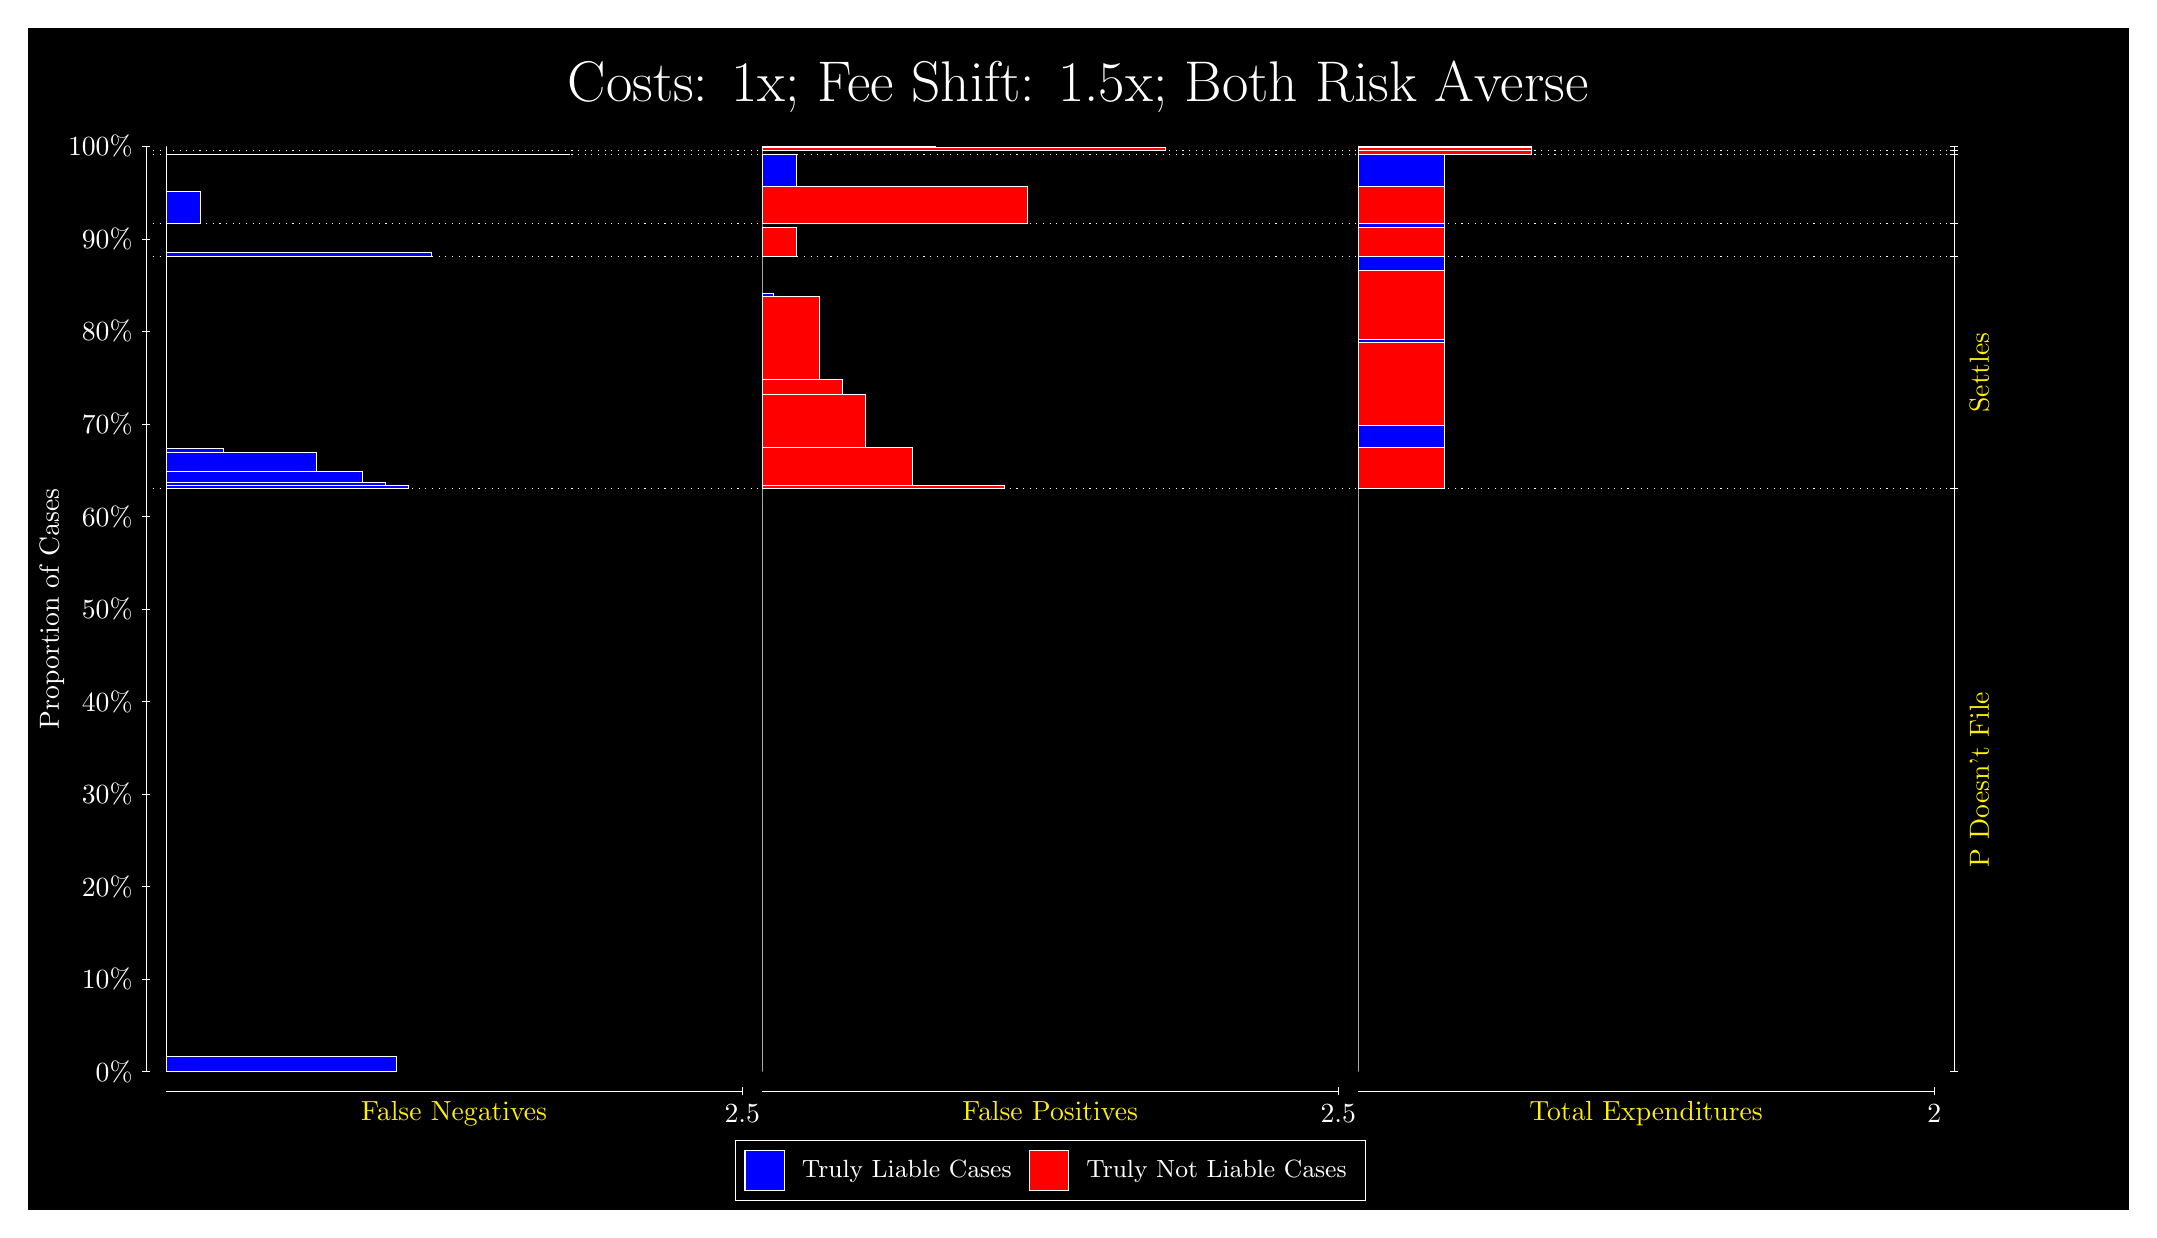
\begin{tikzpicture}
\draw[fill=black] (0,0) rectangle (26.667,15);
\draw[text=white] (0,13.5) rectangle (26.667,15) node[midway] {\huge Costs: 1x; Fee Shift: 1.5x; Both Risk Averse};
\draw[white, very thin] (1.5,1.75) -- (1.5,13.5);
\node[rotate=90, text=white, anchor=center] at (0.3, 7.625) {Proportion of Cases};
\draw[white, very thin] (1.45,1.75) -- (1.55,1.75);
\node[text=white, anchor=east] at (1.45, 1.75) {0\%};
\draw[white, very thin] (1.45,2.925) -- (1.55,2.925);
\node[text=white, anchor=east] at (1.45, 2.925) {10\%};
\draw[white, very thin] (1.45,4.1) -- (1.55,4.1);
\node[text=white, anchor=east] at (1.45, 4.1) {20\%};
\draw[white, very thin] (1.45,5.275) -- (1.55,5.275);
\node[text=white, anchor=east] at (1.45, 5.275) {30\%};
\draw[white, very thin] (1.45,6.45) -- (1.55,6.45);
\node[text=white, anchor=east] at (1.45, 6.45) {40\%};
\draw[white, very thin] (1.45,7.625) -- (1.55,7.625);
\node[text=white, anchor=east] at (1.45, 7.625) {50\%};
\draw[white, very thin] (1.45,8.8) -- (1.55,8.8);
\node[text=white, anchor=east] at (1.45, 8.8) {60\%};
\draw[white, very thin] (1.45,9.975) -- (1.55,9.975);
\node[text=white, anchor=east] at (1.45, 9.975) {70\%};
\draw[white, very thin] (1.45,11.15) -- (1.55,11.15);
\node[text=white, anchor=east] at (1.45, 11.15) {80\%};
\draw[white, very thin] (1.45,12.325) -- (1.55,12.325);
\node[text=white, anchor=east] at (1.45, 12.325) {90\%};
\draw[white, very thin] (1.45,13.5) -- (1.55,13.5);
\node[text=white, anchor=east] at (1.45, 13.5) {100\%};

\draw[white, very thin] (24.457,1.75) -- (24.457,13.5);
\draw[white, very thin] (24.407,1.75) -- (24.507,1.75);
\node[anchor=west] at (24.407, 1.75) {};
\draw[white, very thin] (24.407,9.1577) -- (24.507,9.1577);
\node[anchor=west] at (24.407, 9.1577) {};
\draw[white, very thin] (24.407,12.1) -- (24.507,12.1);
\node[anchor=west] at (24.407, 12.1) {};
\draw[white, very thin] (24.407,12.525) -- (24.507,12.525);
\node[anchor=west] at (24.407, 12.525) {};
\draw[white, very thin] (24.407,13.395) -- (24.507,13.395);
\node[anchor=west] at (24.407, 13.395) {};
\draw[white, very thin] (24.407,13.45) -- (24.507,13.45);
\node[anchor=west] at (24.407, 13.45) {};
\draw[white, very thin] (24.407,13.5) -- (24.507,13.5);
\node[anchor=west] at (24.407, 13.5) {};

\draw[white, very thin, fill=blue] (1.75,1.75) rectangle (4.6775,1.9381);
\draw[white, very thin, fill=red] (1.75,1.9381) rectangle (1.75,9.1577);
\draw[white, very thin, fill=blue] (1.75,9.1577) rectangle (4.8239,9.1995);
\draw[white, very thin, fill=blue] (1.75,9.1995) rectangle (4.5312,9.2352);
\draw[white, very thin, fill=blue] (1.75,9.2352) rectangle (4.2384,9.3759);
\draw[white, very thin, fill=blue] (1.75,9.3759) rectangle (3.6529,9.6168);
\draw[white, very thin, fill=blue] (1.75,9.6168) rectangle (3.3602,9.6194);
\draw[white, very thin, fill=blue] (1.75,9.6194) rectangle (2.4819,9.6647);
\draw[white, very thin, fill=red] (1.75,9.6647) rectangle (1.75,12.1);
\draw[white, very thin, fill=blue] (1.75,12.1) rectangle (5.1167,12.157);
\draw[white, very thin, fill=red] (1.75,12.157) rectangle (1.75,12.525);
\draw[white, very thin, fill=blue] (1.75,12.525) rectangle (2.1891,12.932);
\draw[white, very thin, fill=red] (1.75,12.932) rectangle (1.75,13.395);
\draw[white, very thin, fill=blue] (1.75,13.395) rectangle (6.8732,13.399);
\draw[white, very thin, fill=red] (1.75,13.399) rectangle (1.75,13.45);
\draw[white, very thin, fill=red] (1.75,13.45) rectangle (1.75,13.489);
\draw[white, very thin, fill=blue] (1.75,13.489) rectangle (1.75,13.5);
\draw[white, very thin, fill=red] (9.3189,1.75) rectangle (9.3189,8.9696);
\draw[white, very thin, fill=blue] (9.3189,8.9696) rectangle (9.3189,9.1577);
\draw[white, very thin, fill=red] (9.3189,9.1577) rectangle (12.393,9.192);
\draw[white, very thin, fill=red] (9.3189,9.192) rectangle (11.515,9.1946);
\draw[white, very thin, fill=red] (9.3189,9.1946) rectangle (11.222,9.6728);
\draw[white, very thin, fill=red] (9.3189,9.6728) rectangle (10.636,10.353);
\draw[white, very thin, fill=red] (9.3189,10.353) rectangle (10.344,10.546);
\draw[white, very thin, fill=red] (9.3189,10.546) rectangle (10.051,11.593);
\draw[white, very thin, fill=blue] (9.3189,11.593) rectangle (9.4652,11.639);
\draw[white, very thin, fill=blue] (9.3189,11.639) rectangle (9.3189,12.1);
\draw[white, very thin, fill=red] (9.3189,12.1) rectangle (9.758,12.468);
\draw[white, very thin, fill=blue] (9.3189,12.468) rectangle (9.3189,12.525);
\draw[white, very thin, fill=red] (9.3189,12.525) rectangle (12.686,12.988);
\draw[white, very thin, fill=blue] (9.3189,12.988) rectangle (9.758,13.395);
\draw[white, very thin, fill=red] (9.3189,13.395) rectangle (9.3189,13.445);
\draw[white, very thin, fill=blue] (9.3189,13.445) rectangle (9.3189,13.45);
\draw[white, very thin, fill=red] (9.3189,13.45) rectangle (14.442,13.489);
\draw[white, very thin, fill=blue] (9.3189,13.489) rectangle (11.515,13.5);
\draw[white, very thin, fill=red] (16.888,1.75) rectangle (16.888,8.9696);
\draw[white, very thin, fill=blue] (16.888,8.9696) rectangle (16.888,9.1577);
\draw[white, very thin, fill=red] (16.888,9.1577) rectangle (17.986,9.6728);
\draw[white, very thin, fill=blue] (16.888,9.6728) rectangle (17.986,9.9616);
\draw[white, very thin, fill=red] (16.888,9.9616) rectangle (17.986,11.009);
\draw[white, very thin, fill=blue] (16.888,11.009) rectangle (17.986,11.05);
\draw[white, very thin, fill=red] (16.888,11.05) rectangle (17.986,11.924);
\draw[white, very thin, fill=blue] (16.888,11.924) rectangle (17.986,12.1);
\draw[white, very thin, fill=red] (16.888,12.1) rectangle (17.986,12.468);
\draw[white, very thin, fill=blue] (16.888,12.468) rectangle (17.986,12.525);
\draw[white, very thin, fill=red] (16.888,12.525) rectangle (17.986,12.988);
\draw[white, very thin, fill=blue] (16.888,12.988) rectangle (17.986,13.395);
\draw[white, very thin, fill=red] (16.888,13.395) rectangle (19.083,13.445);
\draw[white, very thin, fill=blue] (16.888,13.445) rectangle (19.083,13.45);
\draw[white, very thin, fill=red] (16.888,13.45) rectangle (19.083,13.489);
\draw[white, very thin, fill=blue] (16.888,13.489) rectangle (19.083,13.5);
\draw[white, dotted] (1.5,9.1577) -- (24.457,9.1577);
\draw[white, dotted] (1.5,12.1) -- (24.457,12.1);
\draw[white, dotted] (1.5,12.525) -- (24.457,12.525);
\draw[white, dotted] (1.5,13.395) -- (24.457,13.395);
\draw[white, dotted] (1.5,13.45) -- (24.457,13.45);
\draw[white, very thin] (1.75,1.5) -- (9.0689,1.5);
\node[text=yellow, anchor=north] at (5.4094, 1.5) {False Negatives};
\draw[white, very thin] (9.0689,1.45) -- (9.0689,1.55);
\node[text=white, anchor=north] at (9.0689, 1.45) {2.5};

\draw[white, very thin] (9.3189,1.5) -- (16.638,1.5);
\node[text=yellow, anchor=north] at (12.978, 1.5) {False Positives};
\draw[white, very thin] (16.638,1.45) -- (16.638,1.55);
\node[text=white, anchor=north] at (16.638, 1.45) {2.5};

\draw[white, very thin] (16.888,1.5) -- (24.207,1.5);
\node[text=yellow, anchor=north] at (20.547, 1.5) {Total Expenditures};
\draw[white, very thin] (24.207,1.45) -- (24.207,1.55);
\node[text=white, anchor=north] at (24.207, 1.45) {2};

\node[text=yellow, centered, rotate=90] at (24.777, 5.4539) {P Doesn't File};
\node[text=yellow, centered, rotate=90] at (24.777, 10.629) {Settles};





\draw (12.978300999999998,1.5) node[draw=none] (baseCoordinate) {};
\begin{scope}[align=center]
        \matrix[scale=0.5, draw=white, below=0.5cm of baseCoordinate, nodes={draw}, column sep=0.1cm]{
            \node[rectangle, draw, minimum width=0.5cm, minimum height=0.5cm, fill=blue] {}; &
            \node[draw=none, font=\small, text=white] (B) {Truly Liable Cases}; &
            \node[rectangle, draw, minimum width=0.5cm, minimum height=0.5cm, fill=red] {}; &
            \node[draw=none, font=\small, text=white] (B) {Truly Not Liable Cases}; \\
            };
\end{scope}

\end{tikzpicture}
\end{document}